\begin{frame}{Manhattan / Taxicab Distance}
   \begin{center}
     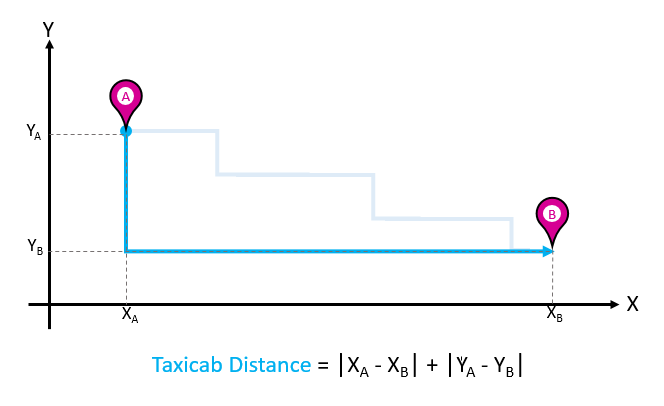
\includegraphics[width=1\textwidth]{figs/taxicab.png}
   \end{center}
\end{frame}

\begin{frame}{A Motivating Puzzle}
  \begin{itemize} 
    \item <+-> Given any $n$ points in any dimension for any $n$,
      compute the $\binom{n}{2}$ Manhattan distances between each pair
      of points. 
      \vs
    \item <+-> Raise each distance to the $2/3$ power.
      \vs
    \item <+-> The result is always a Manhattan distance! 
  \end{itemize}
\end{frame}

\begin{frame} {Why?}
   \begin{center}
     
\includegraphics[width=1\textwidth]{figs/why.jpg}
   \end{center}
\end{frame}
\begin{frame}{A Simple Example}
  \begin{itemize}
    \item <+-> Given $3$ points on a line at at $0, 1$ and $2$, compute
      Manhattan distances between each pair of points.
      \vs
    \item <+-> Raise each distance to the $2/3$ power.
      \vs
    \item <+-> Find $3$ points whose Manhattan distances match these
      powered distances!
  \end{itemize}
\end{frame}

\begin{frame}{A Simple Example}
  \begin{itemize}
    \item <+-> Pairwise distances: $1, 1, 2$.
      \vs
    \item <+-> Powered distances: $1, 1, 2^{2/3}$.
      \vs
    \item <+-> \begin{align}
      & a = \left(\frac{1}{2} + \frac{2^{2/3}}{4}\:,\enspace
      \frac{1}{2}-\frac{2^{2/3}}{4}\right)\nonumber \\
      & b = (0, 0) \nonumber \\
      & c=\left(\frac{1}{2}-\frac{2^{2/3}}{4}\:,\enspace
      \frac{1}{2}+\frac{2^{2/3}}{4}\right). \nonumber
    \end{align}
  \end{itemize}
\end{frame}

\begin{frame}
    \textbf{Definition:} The function $f(x) = x^{2/3}$ \textbf{sends}
  Manhattan distances to Manhattan distances.
\end{frame}

\begin{frame}{The Core Mystery of our Talk}
  \begin{itemize} 
    \item <+-> 
      Why does $x^{2/3}$ send Manhattan distances to
      Manhattan distances?
  \end{itemize}
%  \pause
%   \begin{center}
%     
\includegraphics[width=0.3\textwidth]{figs/mysterybox.jpg}
%   \end{center}

\end{frame}


